%% Chapter 6 %%%
\chapter{Различия в значимости $\neq$ значимые различия}
\label{chp6}

``Мы сравнили лекарство А и Б с действием плацебо. Лекарство А показало значительные улучщения, по сравнению с плацебо, в то время как лекарство Б не имело никаких статистически значимых преимуществ. Следовательно, лекарство А лучше лекарства Б''.

Мы слышим это постоянно. Таким образом легко сравнивать медикаменты, хирургические вмешательства, терапии и экспериментальные результаты. Это просто. И кажется, что это имеет смысл.

Тем не менее, разница в значимости не всегда даёт значимую разницу. \cite{gelman_difference_2006}

Представьте себе исследование, сравнивающее питание моржей. Одну группу моржей кормят обычной едой, в то время как две другие группы питаются неким новым, более питательным кормом. Исследователи взвешивают моржей через месяц и обнаруживают: питательный корм А стал причиной того, что у моржей вес увеличился на 25 кг больше, чем у тех, кто питался обычным кормом, в то время как питательный корм Б увеличил вес моржей лишь на 10 кг. 

Мы хотим узнать, какой средний вес стоит ожидать у каждой из групп моржей. Если мы будем кормить этими тремя типами кормов всех моржей в мире, какой будет средний вес моржей? У нас, к сожалению, на так уж и много моржей, поэтому на этот вопрос будет сложно ответить - все моржи разнятся между собой, и могут набирать вес и по другим причинам, помимо корма (возможно, мужские особи увеличиваются в размерах специально к началу купального сезона). Имея в виду это разнообразие, мы подсчитали, что эффект корма Б статистически незначим: различия между моржами настолько велики, что невозможно сделать вывод о том, что увеличение веса на 10 кг было вызвано именно этим кормом. В то время, как корм А был причиной статистически значимого набора веса, и, по-видимому, эффективен. 

Исследователи могут сделать вывод о том, что ``корм А вызвал статистически значимое увеличение веса, в то время как корм Б - нет; очевидно, что корм А более питательный, чем корм Б.'' Люди, ухаживающие за моржами, могут прочитать эту статью и начнут использовать корм А для питания больных моржей или тех, кто имеет недовес, поскольку этот корм более эффективен.

Но действительно ли он эффективней? Не обязательно.

Поскольку у нас ограниченные данные, они будут иметь погрешности. Мы можем рассчитать, какие результаты будут согласованы с нашими данными: например, ``истинный'' эффект диеты А может давать, в результате, набор веса в 35 или 17 кг, и вполне вероятно, что на нашей небольшой выборке моржей мы увидим действие этого эффекта. Сбор большего количества данных помог бы нам более точно определить размер истинного эффекта.

У статистиков есть инструменты, позволяющие вычислить такую ошибку. Если мы подсчитаем неопределенность каждого из наших инструментов, мы, вероятно, сможем считать вполне убедительным вывод о том, что эффективность обоих кормов была одинакова. Диета Б имеет статистически незначимый эффект, поскольку вполне правдоподобно то, что он вызывает набор веса в 0 кг, равно как и то, что он приводит к набору веса в 20 кг, и просто наша выборка состоит из слишком худых моржей. Схожим образом, вполне вероятно то, что диета А приводит к набору веса в 20 кг и мы просто составили выборку из необычно прожорливых моржей. Мы не можем быть ни в чем уверены без дополнительных данных.


Наших данных недостаточно для того, чтобы сделать вывод о наличии статистически значимых различий между кормами А и Б. В то время как один корм даёт статистически значимые результаты, а другой - нет, статистически значимых различий между ними нет. Они могут быть оба одинаково эффективны, просто нужно быть осторожным при сравнении значимости двух результатов. Если Вы хотите сравнить два лекарства или эффекта, сравнивайте их напрямую. 

Современная литература и новостные ленты изобилуют примерами такой ошибки. Например, огромная часть статей по нейронаукам ее допускает.\cite{nieuwenhuis_erroneous_2011} Возможно, вы помните исследование, опубликованное несколько лет назад, предполагающее то, что люди, имеющие большее количество биологически старших братьев, в большей степени склонны быть гомосексуалистами.\cite{bogaert_biological_2006} Каким образом авторы пришли к такому выводу? И почему, речь шла именно о старших братьях, а не сёстрах?   

Авторы объясняли свой вывод тем, что они провели анализ различных факторов и их влияния на гомосексуальность. Только количество старших братьев имело статистически значимый эффект - количество старших сестёр или небиологических старших братьев не имели статистически значимых эффектов. 

Но, как мы уже видели, это совершенно не гарантирует, что существует значимые различия между эффектами наличия старших братьев или старших сестёр. В действительности, если более пристально взглянуть на данные, можно увидеть, что статистически значимых различий между эффектами наличия старших братьев или старших сестёр просто нет. К сожалению, в статье не было опубликовано достаточное количество данных, чтобы провести прямой подсчет.\cite{gelman_difference_2006}



\section{Когда упускаются значимые различия}
\label{chp6:significantdiffmissed}

На эту проблему можно посмотреть и с другой стороны. Ученые обычно судят о наличии значимых различий буквально на глаз, используя графики наподобие этому:



\newpage % делаем разрыв, чтобы картинка была первой на след странице

%%%%%%%%%%%%%% figure 8 %%%%%%%%%%%%%%%%%%5
\begin{figure}[h!]
    \centering
    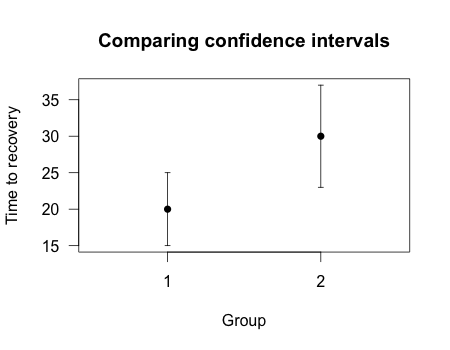
\includegraphics[width=0.5\textwidth]{confidence}
    \caption{Сравнение доверительных интервалов, по оси абсцисс - группы, по оси ординат - время до выздоровления}
    \label{fig5:confidence}
\end{figure}
%%%%%%%%%%%%%%% end of figure %%%%%%%%%%%%%%%%%%%

Представьте, что две нарисованные точки означают примерно оцененное время до выздоравления от некой болезни для двух различных групп пациентов, каждая из которых состоит из десяти пациентов. А эти границы ошибки (линии) могут представлять собой три различные характеристики:

\begin{enumerate}

\item Стандартное отклонение измерений. Подсчитайте разницу между каждым измерением и средним значением, возведите в квадрат эти разницы, а затем подсчитайте среднее значение квадратов и извлеките квадратный корень из получившегося числа. Это и будет стандартное отклонение данной величины и оно измеряет разброс значений по отношению к среднему.

\item Стандартная ошибка какой-либо оценки. Например, возможно, что границы ошибки представляют собой стандартную ошибку среднего. Если бы я решил провести измерения на  множестве различных выборок пациентов, каждая из которых состояла бы из $n$ человек, я могу примерно оценить, что 68\% средних значений времени, требуемого для восстановления, из тех, что я измерил, будут находится в пределах одной стандартной ошибки ``настоящего'' среднего значения времени, необходимого для восстановления. (В случае оценивания средних, стандартная ошибка равна стандартному отклонению, делённому на квадратный корень количества измерений, таким образом, оценка становится тем лучше, чем больше у вас данных, но не слишком быстро.) Многие статистические методы, как, например, регрессия по методу наименьших квадратов, предоставляют оценку стандартной ошибки.   

\item Доверительные интервалы какой-либо оценки. Доверительный интервал уровня 95\%создан математически для того, чтобы включать истинное значение 95 из 100 случайных величин, поэтому в его диапазон входят примерно по два стандартных отклонения в каждом направлении. (Это может быть не совсем верно для более сложных статистических моделей.)  

\end{enumerate}  

Эти три показателя различаются. Стандартное отклонение - это простое измерение моих данных, оно говорит мне о том, как статистическая характеристика, например среднее или наклон наиболее подходящей линии, будет изменяться, если я возьму большое количество пациентов. Доверительный интервал - схожая характеристика, дополнительно гарантирующая, что 95\% доверительных интервалов уровня 95\% должны содержать ``истинное'' значение. 

На графике выше можно увидеть два частично совпадающих доверительных интервала уровня 95\%. Многие ученые, увидев это, сделают вывод об отсутствии статистически значимых различий между группами. В конце концов, группы 1 и 2 \emph{могут и не} различаться - среднее время до восстановления после болезни может быть 25 в обеих группах, нампример, а различия могли проявиться потому что группе 1 в этот раз просто повезло. Но означает ли это, что различие статистически незначимо? Каково будет \emph{\hyperref[chp2:pvalues]{p-значение}}?

В данном случае, $p < 0,05$. Таким образом, существует статистически значимое различие между группами, несмотря на то, что доверительные интервалы частично совпадают.\footnote{Это было подсчитано с использованием t-критерия Стьюдента для независимых выборок, основываясь на стандартной ошибке в 2,5 в группе 1 и 3,5 в группе 2.}

К сожалению, многие ученых пропускают этап тестирования гипотез и просто присматриваются к графикам, чтобы увидеть, пересекаются ли доверительные интервалы. Это даже более консервативный способ - получить результат при котором доверительные интервалы не пересекаются сродни получению $p < 0,01$ в некоторых ситуациях.\cite{schenker_judging_2001} Легко утверждать, что два измерения статистически не различаются в то время, как на самом деле различия есть.  

Противоположно этому, сравнение измерений путем сравнения стандартных ошибок или стандартных отклонений будет также вводить в заблуждение, поскольку границы стандартной ошибки короче границ доверительны интервалов. Два наблюдения могут иметь не пересекающиеся стандартные ошибки, и тем не менее, различия между ними будут статистически не значимыми.

Опрос психологов, нейроученых и медицинских исследователей выявил, что большинство допускают эту простую ошибку помимо того, что многие ученые путают понятия стандартной ошибки, стандартного отклонения и доверительных интервалов. \cite{belia_researchers_2005} Другое исследование научных работ на тему климата обнаружило, что в большинстве статей, сравнивающих 2 группы с использованием границ ошибок, были допущены ошибки.\cite{lanzante_cautionary_2005} Даже вводные учебники по экспериментальной науке, такие как ``Введение в анализ ошибок'', учат студентов принимать решение ``на глаз'', вообще едва упоминая формальную проверку гипотез.   

Конечно, существуют формальные статистические методы, которые создают доверительные интервалы, которые можно сравнивать на глаз, и даже автоматически корректирую множественные сравнения. Например, сравнительные интервалы Гэбриэля легко интерпретировать на глаз. \cite{gabriel_simple_1978}

Частично совпадающие доверительные интервалы не означают, что два значения не различаются статистически. Схожим образом, не пересекающиеся границы стандартных ошибок не означают, что две величины статистически отличаются. Всегда лучше использовать подходящий тест для проверки гипотезы, поверьте, ваш глаз - не самый хороший статистический метод. 